%!TEX program = xelatex
\documentclass[xetex]{beamer}
\usetheme[width=2cm]{PaloAlto}                          %controls the width of the sidebar
\setbeamercolor{frametitle}{bg=blue!80!black}                 %controls the color of the headline
\setbeamercolor{sidebar}{bg=gray!80}                    %controls the color of the sidebar
\setbeamercolor{logo}{bg=gray!80!black}                       %controls the color of the logo area
% \setbeamercolor{section in sidebar}{fg=...}             %color of the active section
% \setbeamercolor{section in sidebar shaded}{fg=...}      %color of the inactive section
% \setbeamercolor{subsection in sidebar}{fg=...}          %color of the active subsection
% \setbeamercolor{subsection in sidebar shaded}{fg=...}   %color of the inactive subsection
\setbeamercolor{title in sidebar}{fg=black}               %color of the presentation title
\setbeamercolor{author in sidebar}{fg=black}              %color of the author
% !TEX root = ../main.tex
\usepackage{hyperref}
\usepackage{float}
\usepackage{graphicx}		% for pdf, bitmapped graphics files
\graphicspath{ {figs/} }
\usepackage{times} 			% assumes new font selection scheme installed
\usepackage{mathtools} 		% assumes mathtools package installed
\usepackage{amssymb}  		% assumes amssymb package installed
\usepackage{amsthm}
\usepackage{caption}
\usepackage{subcaption}
\usepackage{setspace}
\usepackage{tikz}
\usetikzlibrary{positioning}
\usetikzlibrary{patterns}
\usepackage{xcolor}
\usepackage{tabularx,lipsum}
\usepackage{xltxtra}
\usepackage{xgreek}
\usepackage{fontspec}
\usepackage{booktabs}
\setmainfont[Mapping=tex-text]{GFS Didot}
\setsansfont[Mapping=tex-text]{GFS Didot}
\usepackage{xunicode}
\usepackage{fancyvrb}
\usepackage{pifont}
\newcommand{\cmark}{\ding{51}}%
\newcommand{\xmark}{\ding{55}}%
\logo{
\includegraphics[height=0.5cm,keepaspectratio]{RG}}
\title{Συνεισφορά στο Gretl}
\author{Άρης Συνοδινός}
\institute{Τμ. Μηχ/γων Μηχ/κών \& Αερ/γών\\
Ερευνητική Ομάδα Ρομποτικής\\
Πανεπιστήμιο Πατρών\\ \hfill \\{
\includegraphics[width=2cm,keepaspectratio]{RG}}}
\date{\today}

\AtBeginSection[]
{
  \begin{frame}
    \frametitle{Περιεχόμενα}
    \tableofcontents[currentsection]
  \end{frame}
}

\begin{document}

\makeatletter
\begin{frame}[plain]
    \hspace*{-\beamer@leftsidebar}%
    \advance\textwidth by \beamer@leftsidebar\relax
    \beamer@leftsidebar=\z@
    \begin{minipage}{\textwidth}\par%
    \maketitle
    \end{minipage}
\end{frame}
\makeatother

\section{Εισαγωγικά}

\begin{frame}{Λίγα πράγματα για το Gretl}
    \begin{block}{Το χρονικό}
        Η ανάπτυξη του ξεκίνησε το 2000 ενώ η τελευταία σταθερή έκδοση που είναι διαθέσιμη είναι η 1.10.1, που ανακοινώθηκε στις 4/4/2015.
    \end{block}
    \pause
    \begin{exampleblock}{Ο τρόπος}
        Είναι γραμμένο σε C, και χρησιμοποιεί πολλές βιβλιοθήκες ανοιχτού κώδικα (GTK, GMP, LAPACK, Libxml2, FFTW, cURL)
    \end{exampleblock}
    \pause
    \begin{alertblock}{Το μέλλον...}
        Αναπτύσσεται με πολύ αργούς ρυθμούς από πολύ λίγα άτομα!
    \end{alertblock}
\end{frame}

\begin{frame}{Στην περίοδο του χρόνου}
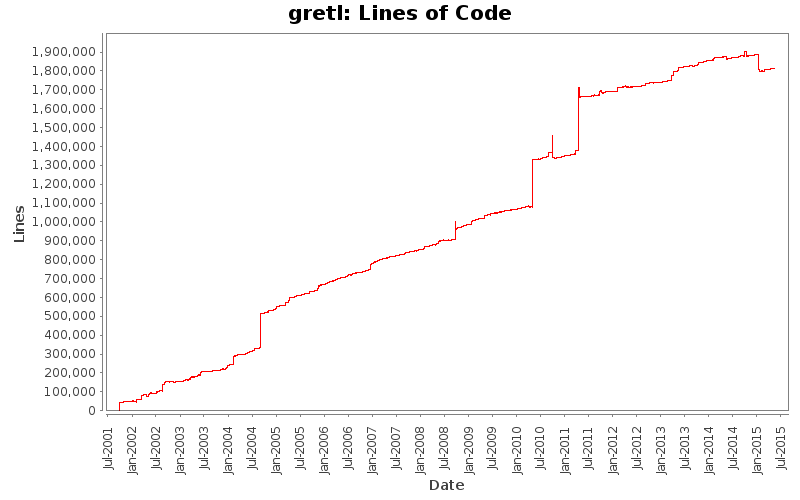
\includegraphics[width=\textwidth]{loc}
\end{frame}

\begin{frame}[fragile]{Ποιοι;}
    \begin{Verbatim}[fontsize=\tiny]
    ---------------------------------------------------------------------
    Author          Changes         Lines of Code       Lines per Change
    ---------------------------------------------------------------------
    allin           57968 (94.7%)   11783051 (93.5%)    203.2
    roadrunner_0    564 (0.9%)      170763 (1.4%)       302.7
    ch_andrade      125 (0.2%)      158437 (1.3%)       1267.4
    svetosch        63 (0.1%)       85874 (0.7%)        1363.0
    artbala         51 (0.1%)       85759 (0.7%)        1681.5
    etpdihei        182 (0.3%)      67023 (0.5%)        368.2
    jacklucchetti   1101 (1.8%)     55884 (0.4%)        50.7
    yi-nung         49 (0.1%)       54169 (0.4%)        1105.4
    f_bresson       36 (0.1%)       39450 (0.3%)        1095.8
    crig            794 (1.3%)      39330 (0.3%)        49.5
    markus_h        7 (0.0%)        18037 (0.1%)        2576.7
    gedranovich     78 (0.1%)       17829 (0.1%)        228.5
    talhayalta      162 (0.3%)      17604 (0.1%)        108.6
    uid64116        30 (0.0%)       1727 (0.0%)         57.5
    ecadrian        23 (0.0%)       746 (0.0%)          32.4
    ---------------------------------------------------------------------
                    Totals          61233 (100.0%)      12595683 (100.0%)
    ---------------------------------------------------------------------
    \end{Verbatim}
\end{frame}

\begin{frame}{Επίσημα}
    \begin{block}{Dependencies}
    Gretl depends on various libraries, as well as the program gnuplot, for parts of its functionality. The table below gives a summary of these dependencies. The link on the left leads to the main site for the package in question (valid as of October, 2011) while the link on the right leads to a search for the package on rpmfind.net.
    \end{block}
\end{frame}

\begin{frame}{Εξαρτήσεις}
    \begin{tabular}{| l | l |}
    \hline
    gtk & provides the gretl GUI\\
    gtksourceview & syntax highlighting\\
    libxml & open and save data files\\
    lapack & linear algebra library\\
    fftw3 & Fast Fourier Transform\\
    gnuplot & generate graphs\\
    GMP & support multiple-precision OLS\\
    libcurl & HTTP protocol\\
    MPFR & additional multiple-precision\\
    readline & editable command line in gretlcli\\
    JSON-GLib & provides for parsing of data\\
    \hline
    \end{tabular}
\end{frame}

\begin{frame}[fragile]{Μερικά στατιστικά του κώδικα}
    \begin{Verbatim}[fontsize=\tiny]
        1114 text files.
        1086 unique files.                                          
         614 files ignored.

    -------------------------------------------------------------------------------
    Language                     files          blank        comment           code
    -------------------------------------------------------------------------------
    C                              281          66374          43888         310702
    Bourne Shell                    24           4620           4398          30300
    C/C++ Header                   170           4888           3379          12242
    m4                              12           1091            313          10857
    make                             8            138             15            582
    XML                              5              6              2            387
    Perl                             3             50             13            366
    DTD                              3             37             14            179
    -------------------------------------------------------------------------------
    SUM:                           506          77204          52022         365615
    -------------------------------------------------------------------------------
    \end{Verbatim}
\end{frame}

\begin{frame}{Η συνταγή της επιτυχίας!}
    \begin{block}{`Πουλώντας' το ΕΛ/ΛΑΚ}
    Αν και το ελεύθερο λογισμικό δεν έχει τιμή, οι αρχές του μάρκετινγκ ισχύουν και για αυτό.
    \end{block}
    \pause
    \begin{enumerate}
    \item Να λειτουργεί σωστά και αποδοτικά \pause \cmark
    \item Να έχει εύχρηστο GUI \pause \cmark
    \item Να είναι καλά τεκμηριωμένο \pause \cmark
    \item Να έχει όμορφη ιστοσελίδα \pause \xmark
    \item Να είναι εύκολο να συνεισφέρουν προγραμματιστές \pause \xmark
    \item Να ακολουθεί τις τεχνολογικές εξελίξεις \pause \xmark
    \end{enumerate}
\end{frame}

\begin{frame}{Λειτουργία - Απόδοση}
	\begin{center}
	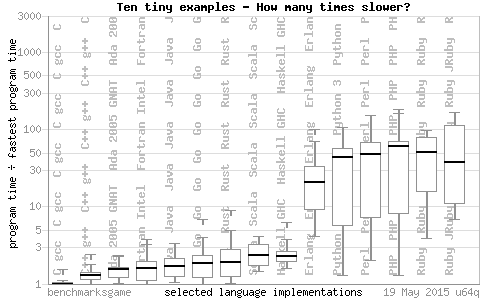
\includegraphics[width=\textwidth]{programming_speed}
	\end{center}
\end{frame}

\begin{frame}{Εύχρηστο GUI}
   \begin{columns}
    \begin{column}{.3\textwidth}
     	\begin{itemize}
		\item tcl/TK
		\item FLTK
		\item QT
		\item GTK+
		\item WxWidgets
		\end{itemize}
    \end{column}
    \begin{column}{.7\textwidth}
     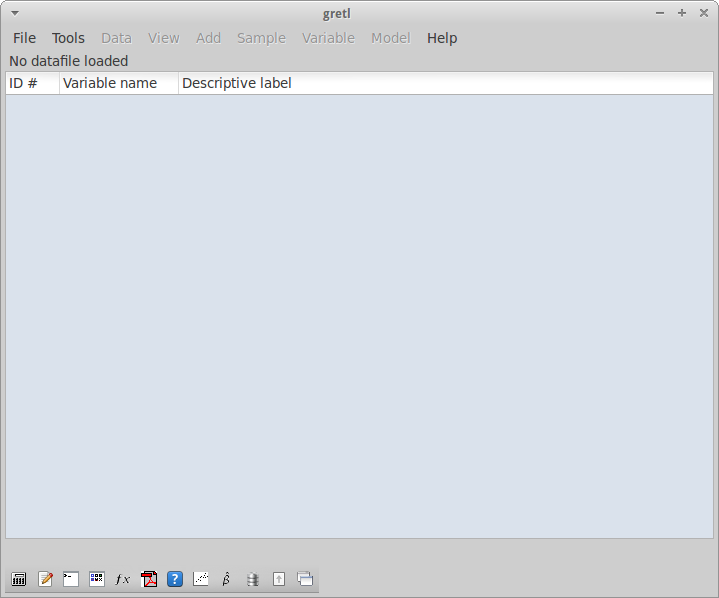
\includegraphics[width=\textwidth]{gretl_gui}
    \end{column}
   \end{columns}
\end{frame}

\begin{frame}{Τεκμηρίωση - Χρήστες!}
	\begin{columns}
    \begin{column}{.5\textwidth}
		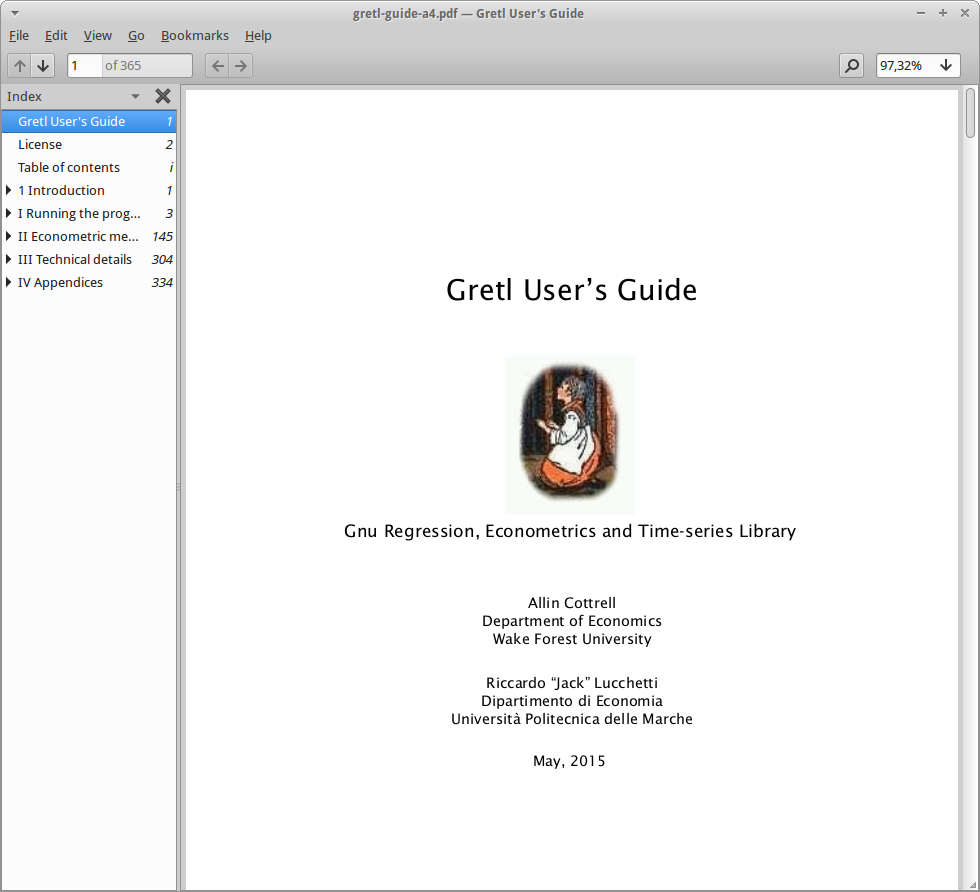
\includegraphics[width=\textwidth]{gretl_guide}
    \end{column}
    \begin{column}{.5\textwidth}
    	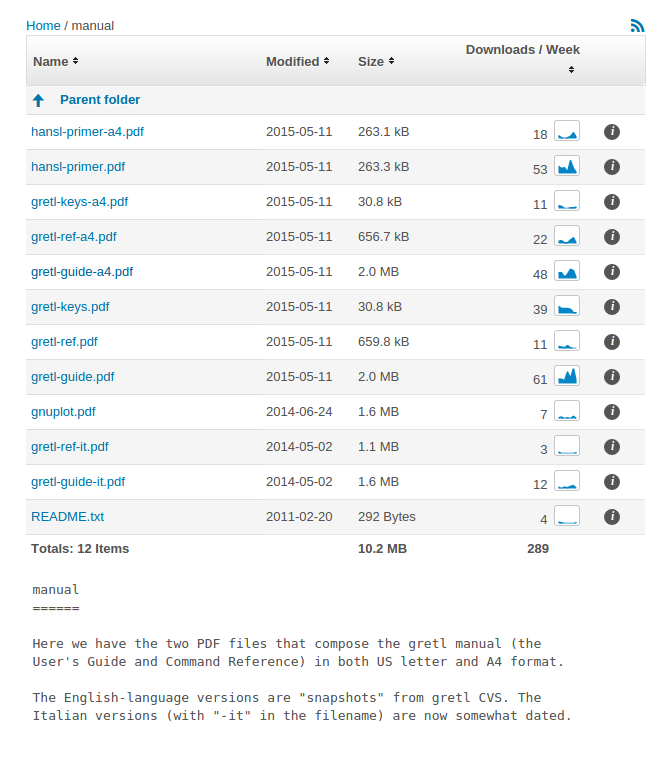
\includegraphics[width=\textwidth]{gretl_docs}
    \end{column}
   \end{columns}
\end{frame}

\begin{frame}{Τεκμηρίωση - Χρήστες!}
	\begin{center}
    	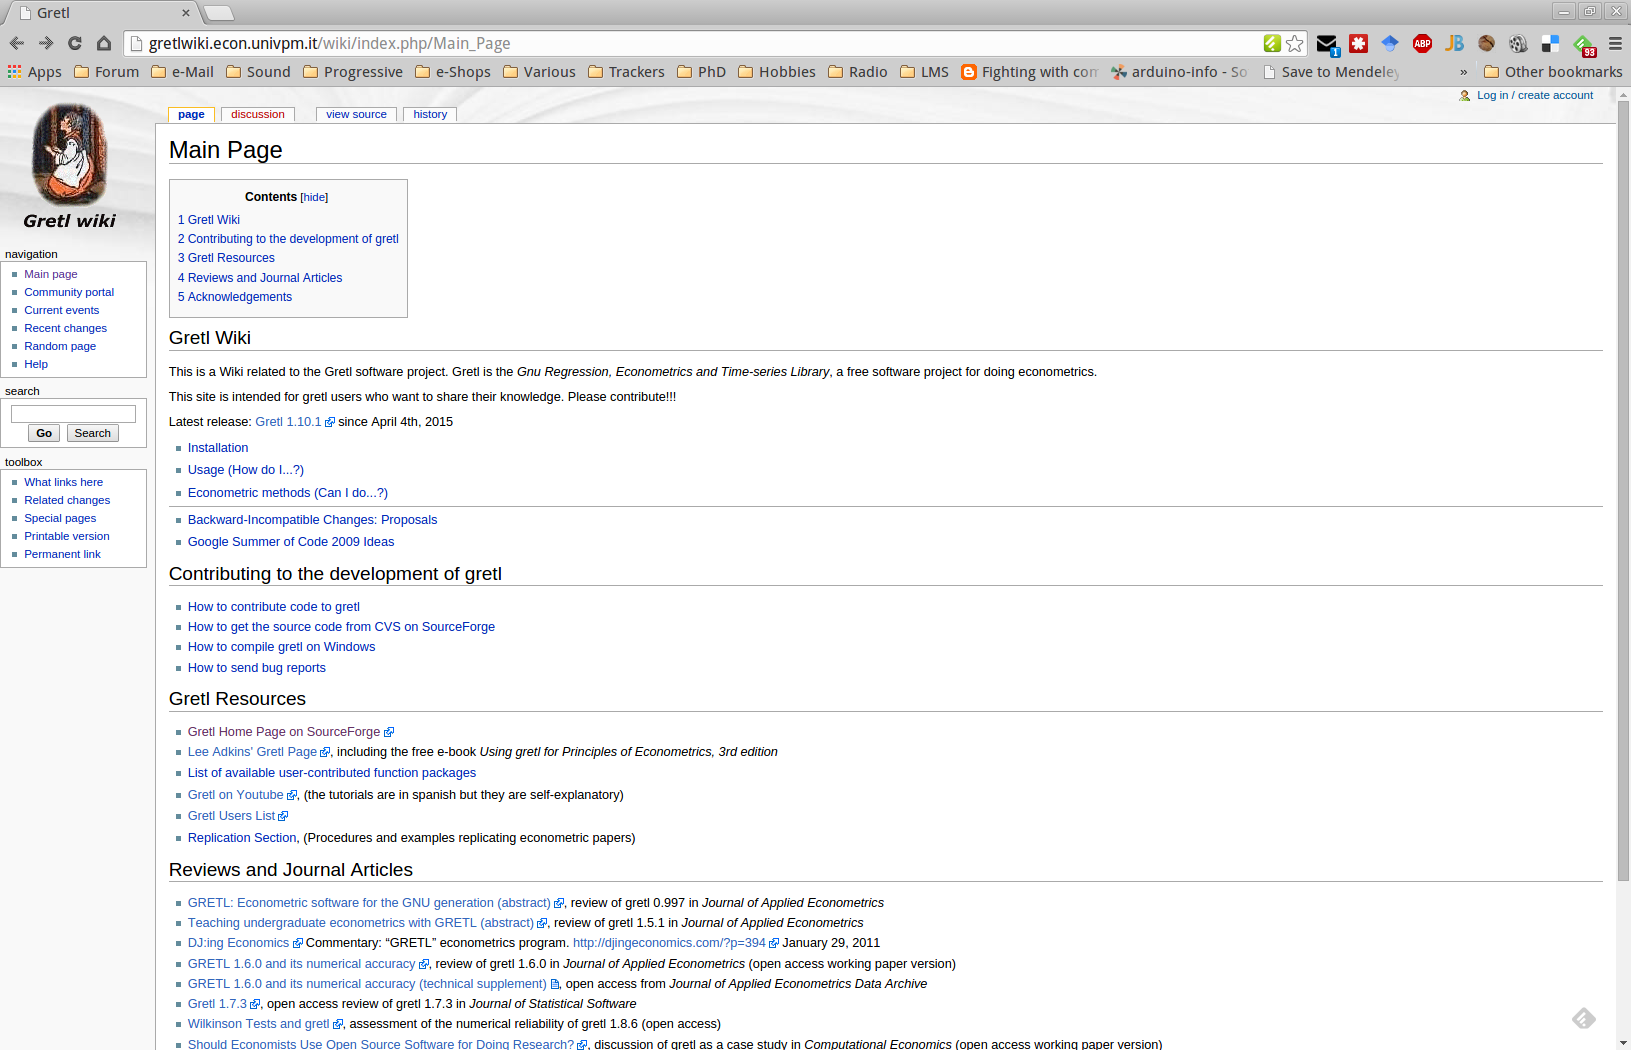
\includegraphics[width=\textwidth]{gretl_wiki}
    \end{center}
\end{frame}

\begin{frame}{Τεκμηρίωση - Προγραμματιστές!}
	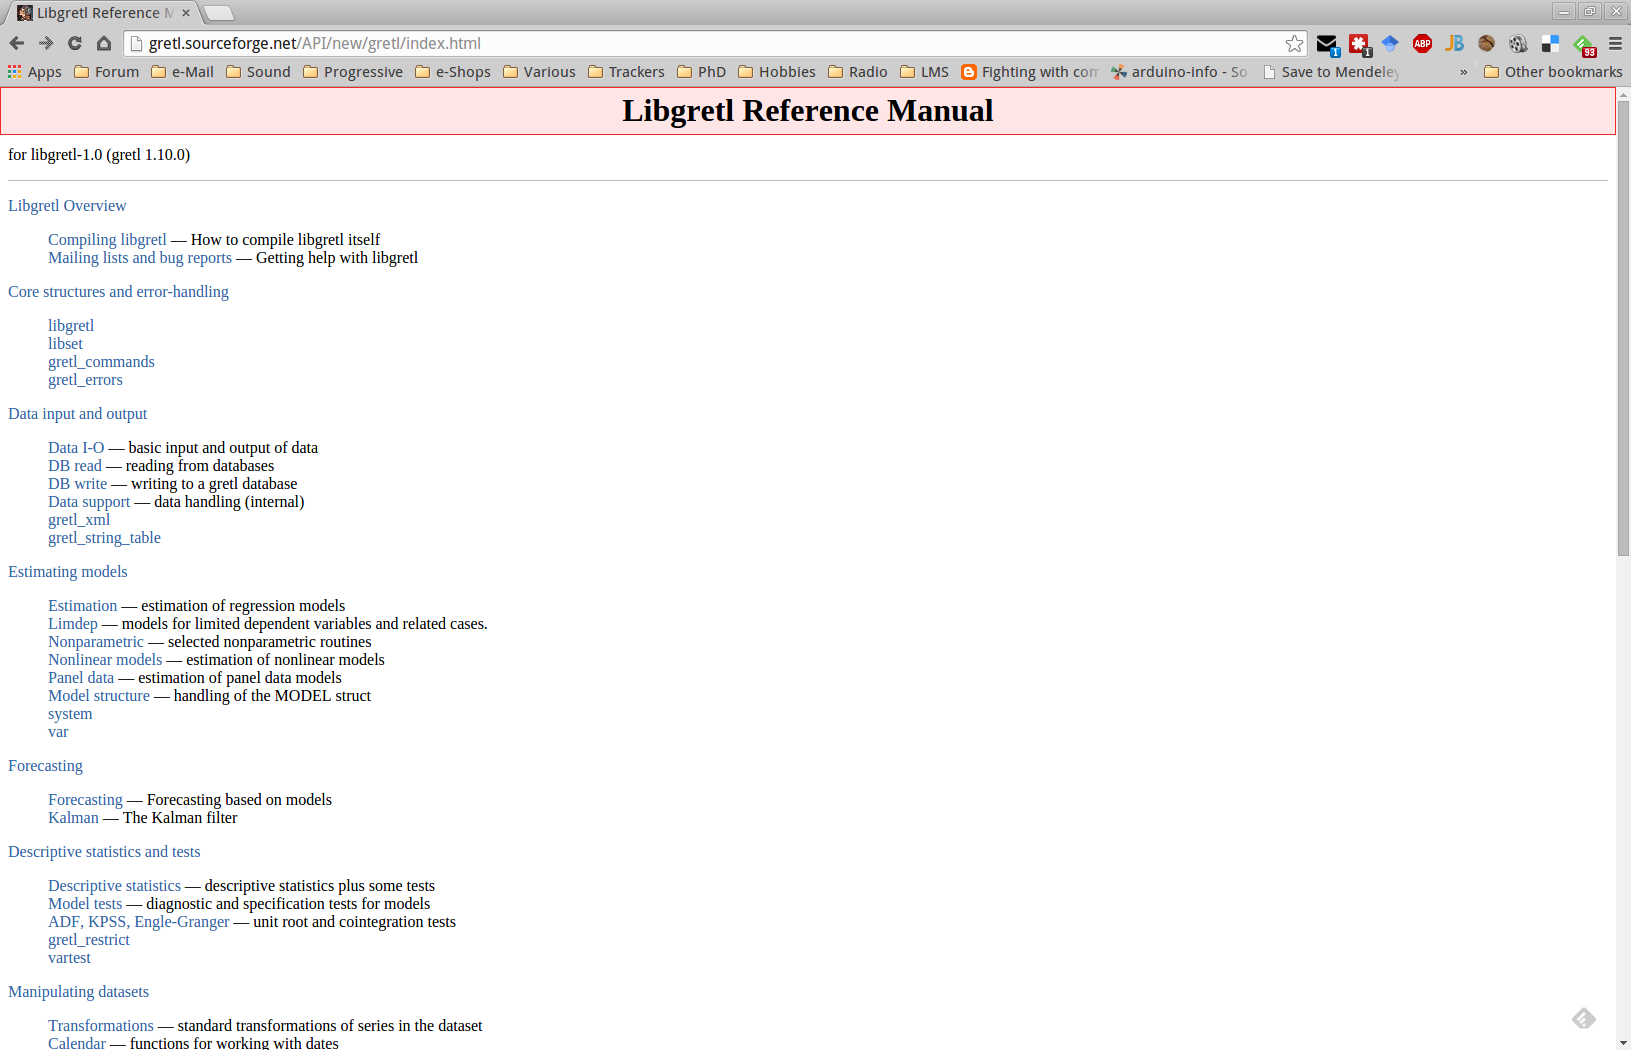
\includegraphics[width=\textwidth]{libgretl_api}
\end{frame}

\begin{frame}{Τεκμηρίωση - Προγραμματιστές!}
    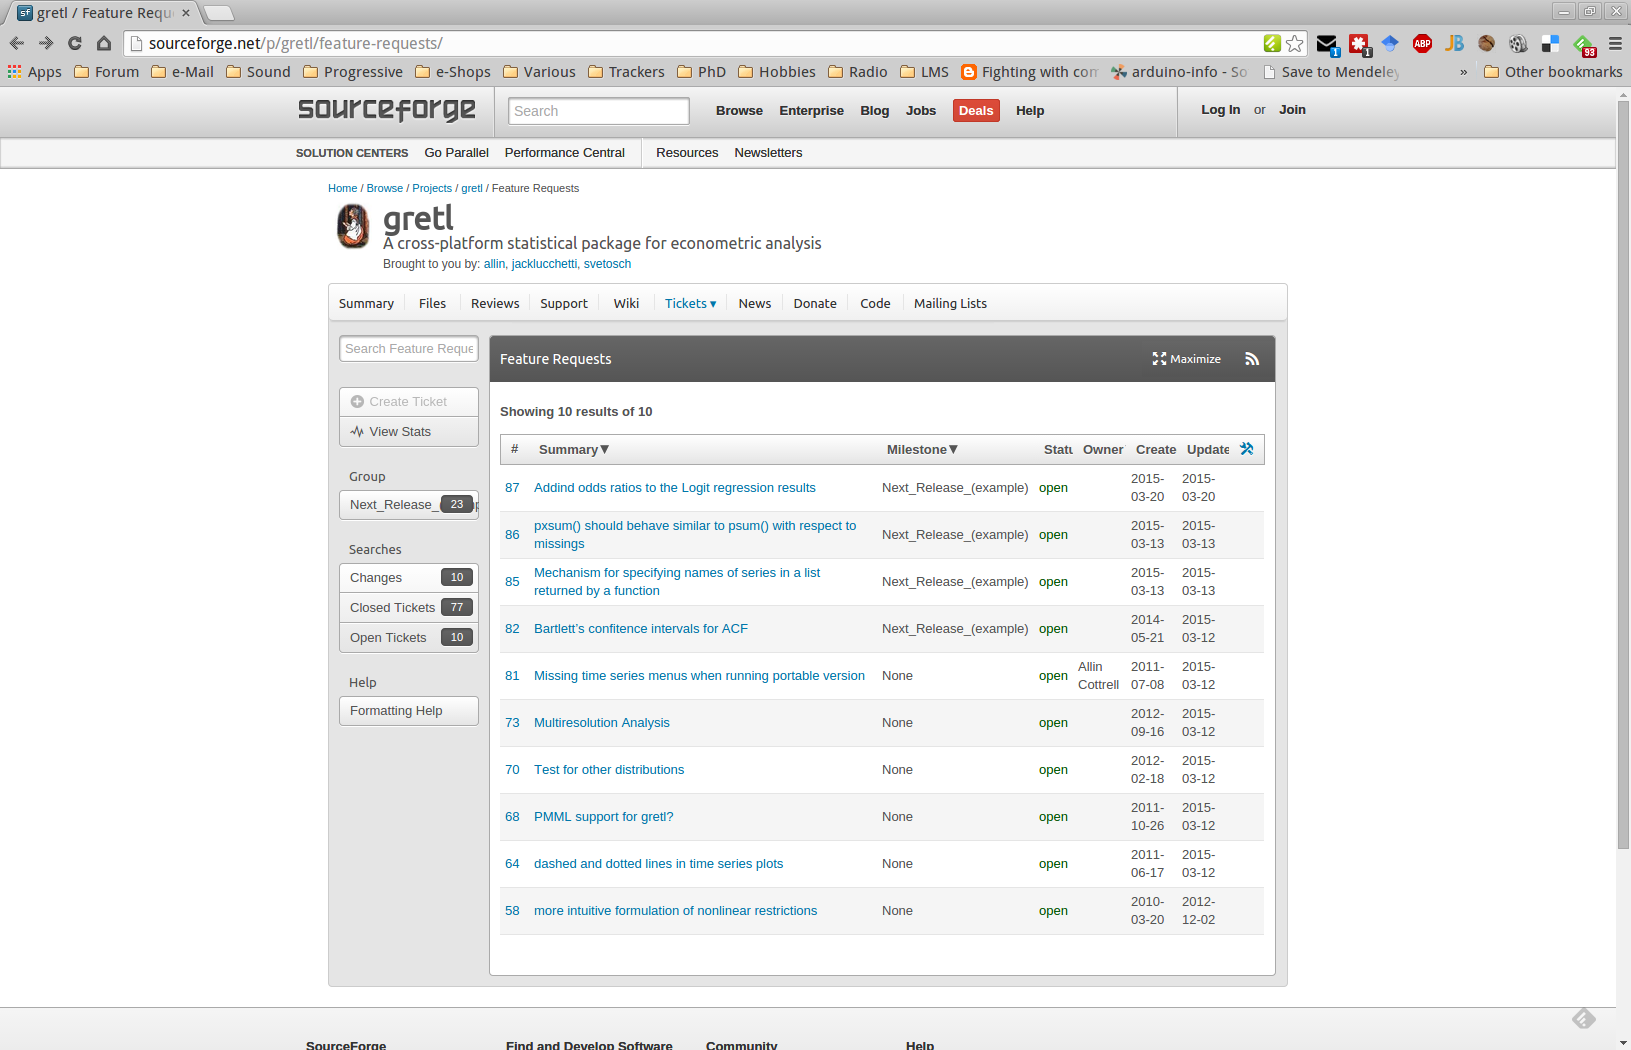
\includegraphics[width=\textwidth]{issue_tracking}
\end{frame}

\section{Συνεισφορά}

\begin{frame}{Γλώσσα Προγραμματισμού}
	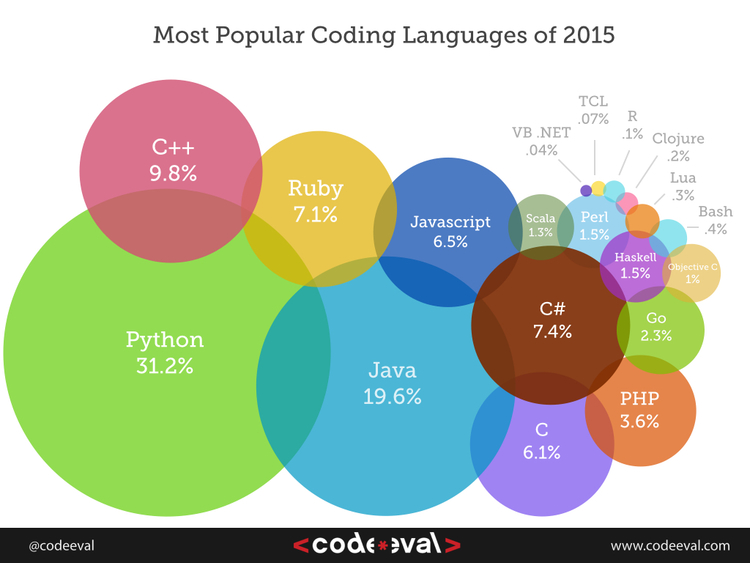
\includegraphics[width=\textwidth]{coding-lan}
\end{frame}

\begin{frame}{Toolchain}
	Τα δημοφιλέστερα cross-platform toolchains
	\begin{itemize}
		\item GNU Autotools
		\item CMake
		\item QMake
		\item SCons
	\end{itemize}
	\begin{center}
		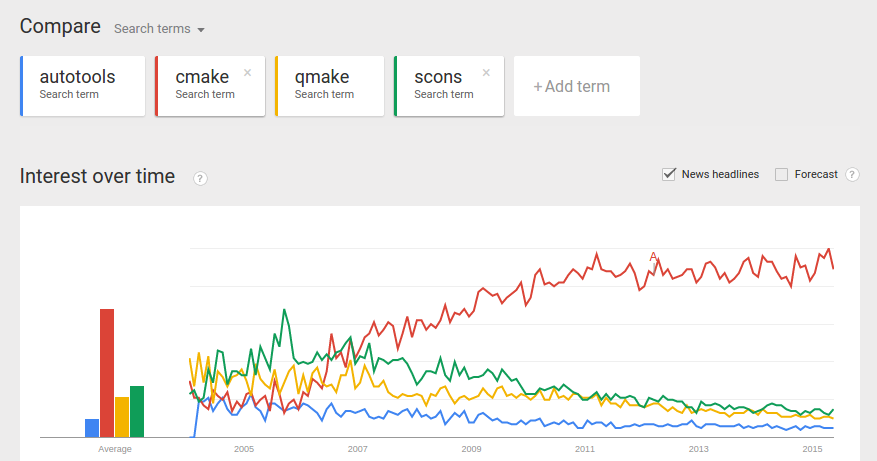
\includegraphics[width=.7\textwidth]{build_tools}
	\end{center}
\end{frame}

\begin{frame}{Version Control Software}
	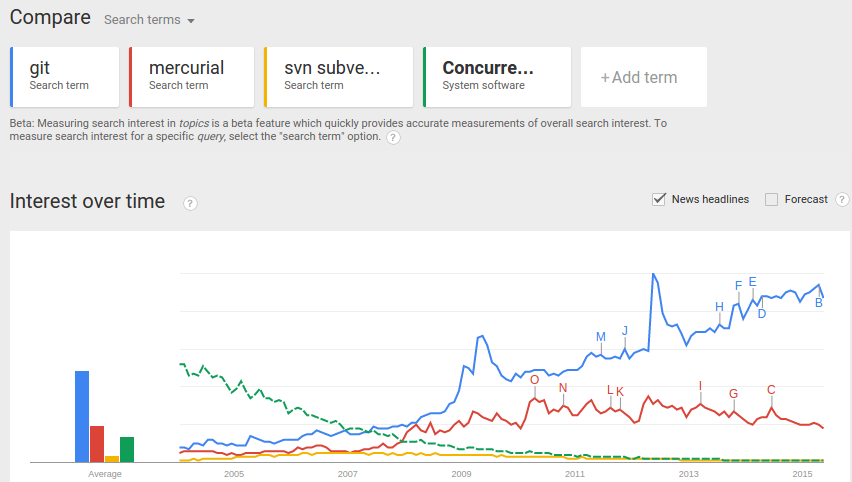
\includegraphics[width=\textwidth]{vcs}
\end{frame}

\begin{frame}{Testing Frameworks}
	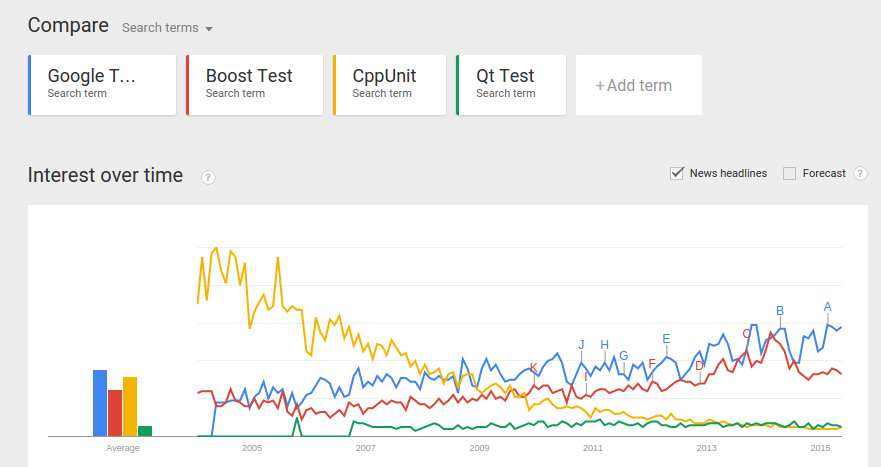
\includegraphics[width=\textwidth]{tests}
\end{frame}

\begin{frame}{Εξέλιξη}
	Νέα γενιά εργαλείων
	\begin{itemize}
		\item Αυτόματη μεταγλώττιση
		\item Διαχείριση εξαρτήσεων
		\item Μεταγλώττιση κατά βήματα
		\item Αναφορές που συσχετίζουν τον πηγαίο κώδικα με το εκτελέσιμο
		\item Επιτάχυνση μεταγλώττισης
		\item Αναφορές που σχετίζονται με την ποιότητα, το περιεχόμενο ή τις επιδόσεις
		\item Αυτόματη τεκμηρίωση
		\item Αναφορές αποσφαλμάτωσης
		\item Έλεγχος αποτελέσματος (Unit Testing)
		\item Αναφορές επιθυμητών χαρακτηριστικών
	\end{itemize}
\end{frame}

\begin{frame}{Continuous Integration}
	\begin{enumerate}[<+->]
	\item Συντήρηση ενός αποθετηρίου
	\item Αυτοματοποίηση της μεταγλώττισης
	\item Αυτοματοποίηση των ελέγχων
	\item Όλοι μπορούν να συνεισφέρουν
	\item Όλες οι συνεισφορές μεταγλωττίζονται και ελέγχονται
	\item Δοκιμές σε πραγματικό περιβάλλον
	\item Ευκολία διαχείρισης των παραδοτέων
	\item Όλοι μπορούν να δουν τα αποτελέσματα
	\item Αυτόματη εγκατάσταση
	\end{enumerate}
\end{frame}

\begin{frame}{Είναι δημοφιλή;}
	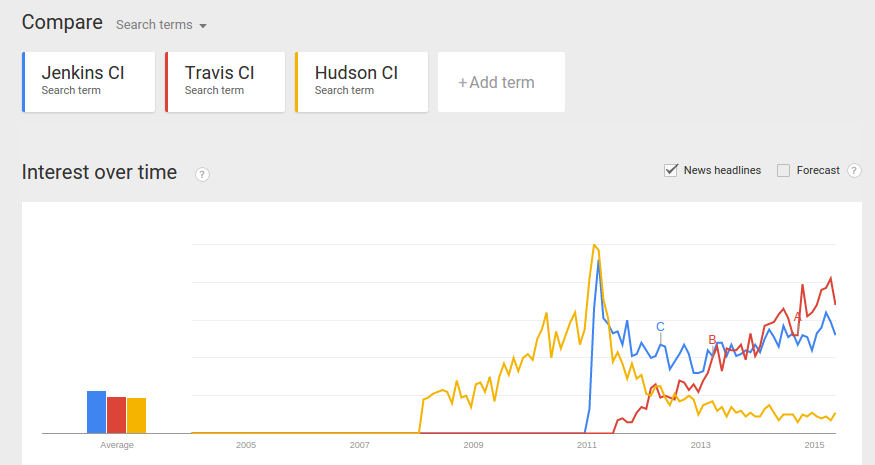
\includegraphics[width=\textwidth]{continuous_integration}
\end{frame}

\begin{frame}{Code Coverage}
	Coveralls.io
	
\includegraphics[width=\textwidth]{coveralls_io}
\end{frame}

\begin{frame}{Αυτόματη εγκατάσταση}
	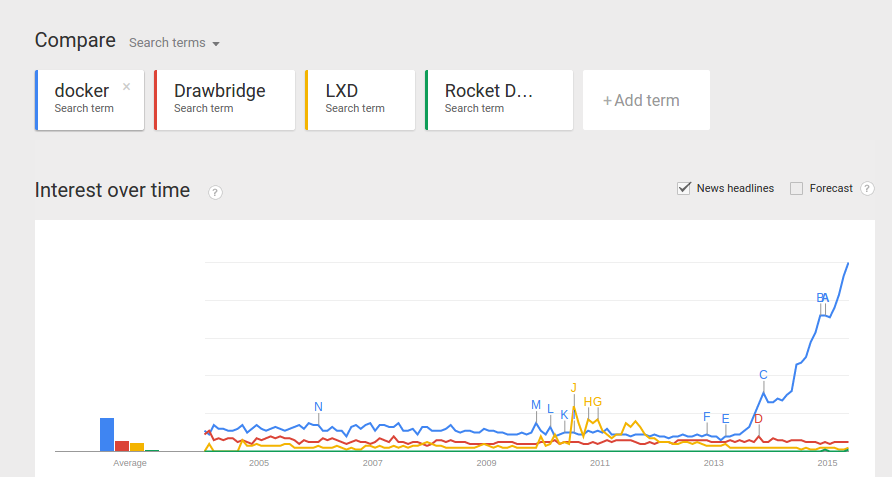
\includegraphics[width=\textwidth]{docker}
\end{frame}

\begin{frame}{Workflow}
	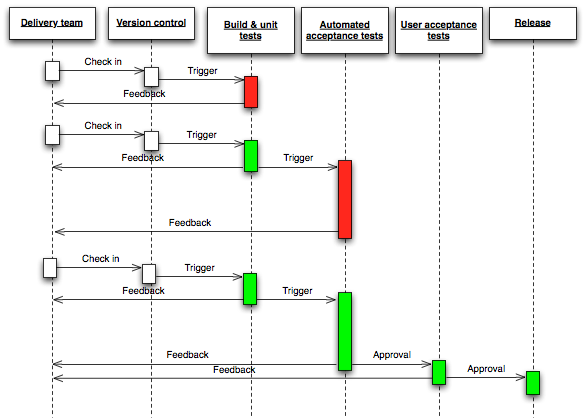
\includegraphics[width=\textwidth]{Continuous_Delivery_process_diagram}
\end{frame}

\begin{frame}{Τελικό αποτέλεσμα}
	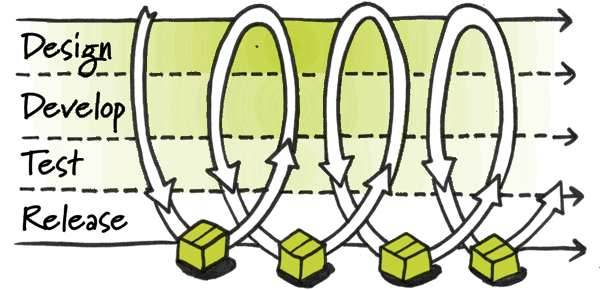
\includegraphics[width=\textwidth]{ddtr}
\end{frame}

\begin{frame}{Github}
	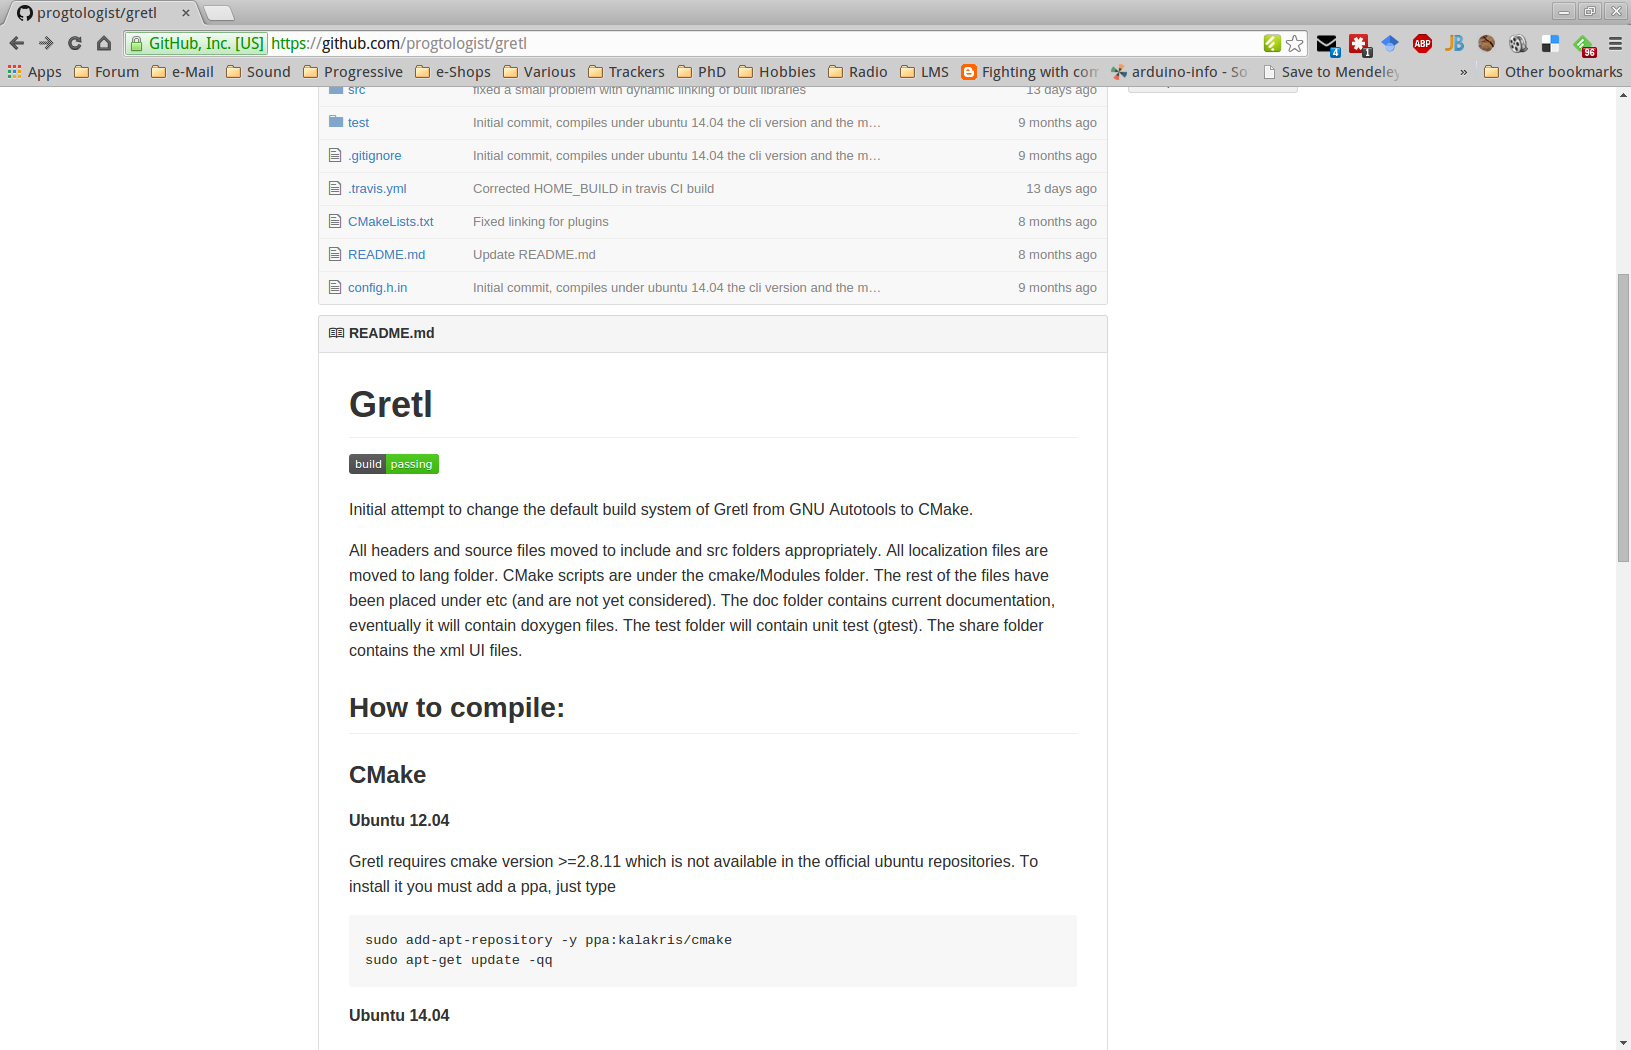
\includegraphics[width=\textwidth]{github_gretl}
\end{frame}

\begin{frame}{Travis}
	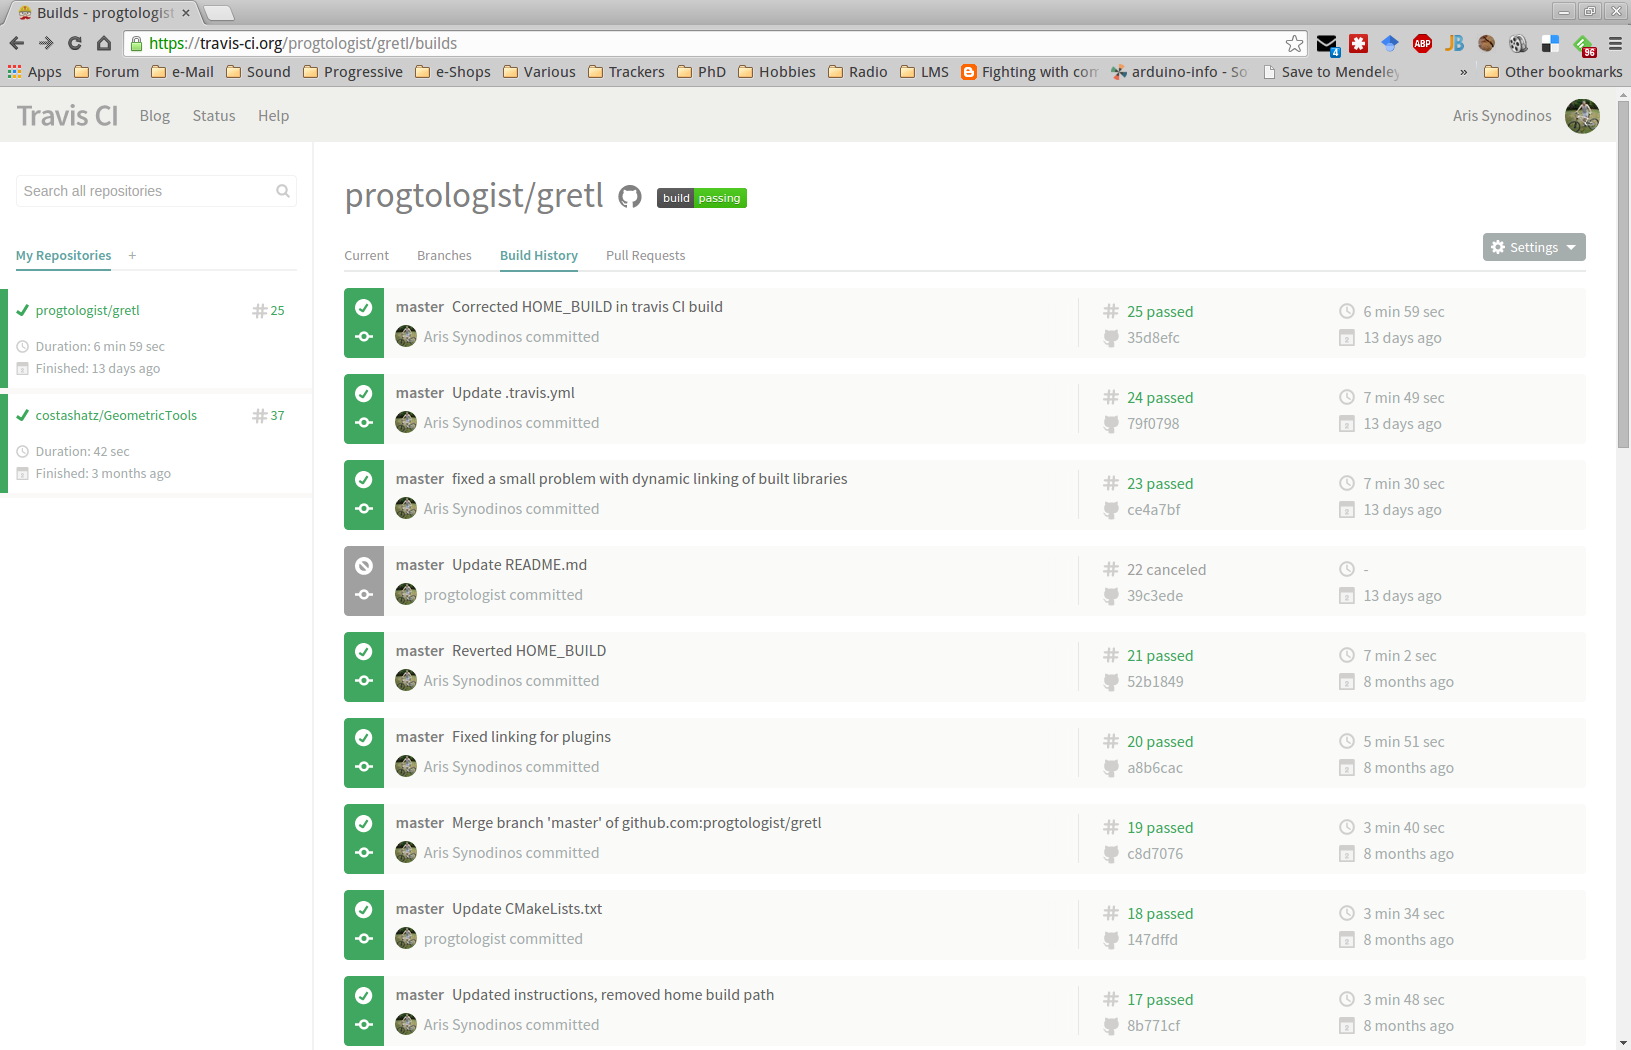
\includegraphics[width=\textwidth]{travis_gretl}
\end{frame}

\begin{frame}{Documentation}
	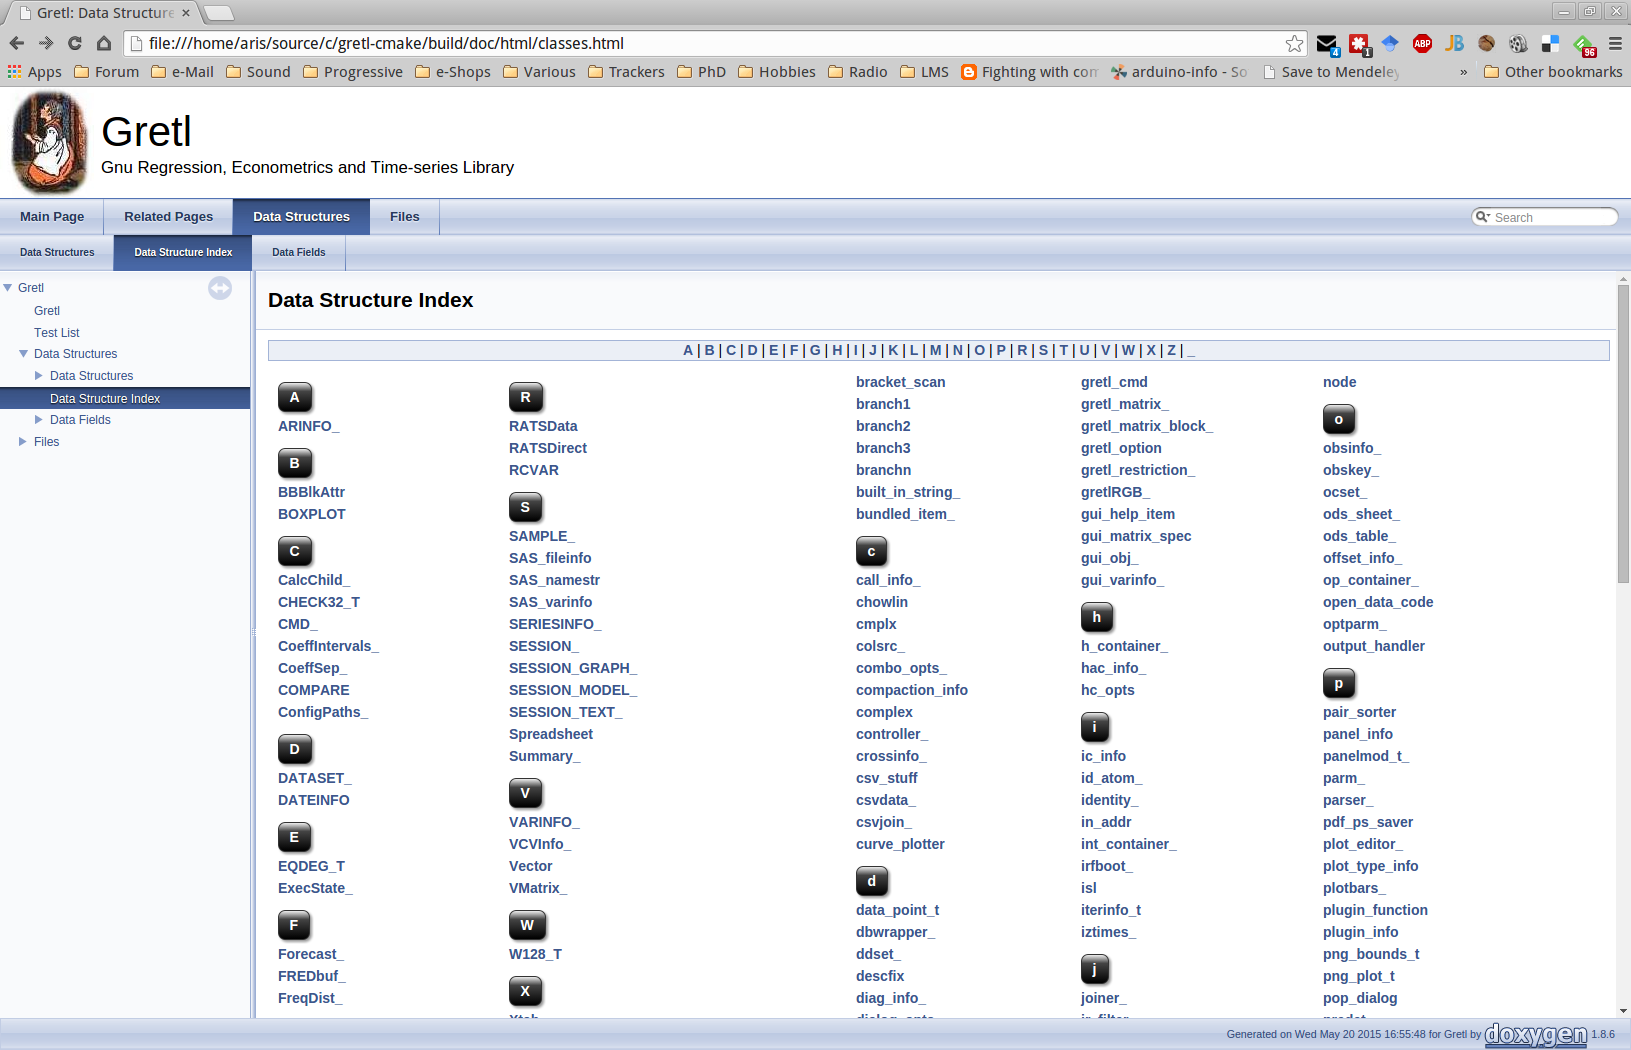
\includegraphics[width=\textwidth]{gretl_doxy}
\end{frame}

\begin{frame}{Απορίες}
	\centering \Huge ?
\end{frame}

\end{document}
